\documentclass{article}


\usepackage{iclr2027_conference,times}
\usepackage[utf8]{inputenc}
\usepackage[T1]{fontenc}
\usepackage{amsmath,amssymb}
\usepackage{graphicx}
\usepackage{booktabs}
\usepackage{xcolor}
\usepackage{subcaption}
\usepackage{float}
\usepackage{hyperref}
\usepackage{url}
\usepackage{caption}

%\iclrfinalcopy

\newcommand{\placeholder}[2][0.7\linewidth]{%
  \fbox{\parbox[c][3.2cm][c]{#1}{\centering\itshape\color{gray} #2}}%
}

\title{Emergent Tool Use in the Hide-and-Seek Environment via an Adaptive Auto-Curriculum}



\author{Anonymous authors\\Paper under double-blind review}

\begin{document}
\maketitle

\begin{abstract}

We study the emergence of coordinated multi-agent strategies in the
quadrant configuration of Openai's hide-and-seek environment. Two teams,
hiders and seekers, are trained purely through self-play under a zero-sum
reward with no additional rewards on specific behaviours. To drive learning we combine
self-play against a pool of past opponents with an adaptive
auto-curriculum, inspired by Deepmind's
Adaptive Agent research. Over the course of training we observe a
sequence of distinct emergent phases: pursuit and evasion, door blocking, seeker ramp use, and a hider ramp-defense strategy. We
monitor the emerge of these phase transitions and, in a controlled
ablation across three random seeds, find that the adaptive curriculum reaches all
four phases faster than a non-adaptive task
sampler and with lower seed-to-seed variance. Relative to the phase onsets
originally reported for the full hide-and-seek environment, our compact
single-scenario setup reaches the final phase roughly 1.3 times
faster (about 3M episodes), while following the same ordering of
emergent behaviours.

\end{abstract}

\section{Introduction}

Multi-agent reinforcement learning can produce sophisticated
behaviour without explicit supervision: as one team improves, it changes the
task faced by the other, producing an autocurriculum
\citep{baker2019emergent}. In the hide-and-seek domain, This process can lead to tools being used even when they were never directly rewarded. In this work we focus
exclusively on the \textbf{quadrant} scenario and inspect what behaviours emerge when this scenario is paired with an adaptive auto-curriculum.

The \textbf{quadrant} scenario places two hiders and two seekers in a square
arena whose corner is walled off into a small room---the ``quadrant''---reachable
only through one or two doorways. During a short preparation phase the seekers are
frozen while the hiders may drag boxes to seal the doorways and reposition the
single ramp; the seekers are then released and try to establish line of sight on a
hider. This layout is deliberately minimal: it isolates the box-and-ramp tool-use
loop that drives emergence without the additional rooms and objects of the full
hide-and-seek environment. To decide \emph{which} door configuration to train on at
each moment, we pair the scenario with an \emph{adaptive auto-curriculum} that
continually re-samples configurations in proportion to their estimated learning
potential (regret), concentrating experience on the configuration the agents are
currently able to make progress on rather than sampling all of them uniformly.

Studying this progression matters because it exemplifies how open-ended
competitive pressure can bootstrap increasingly sophisticated skills without any
reward for the skills themselves, offering a controllable microcosm of
curriculum-driven emergence. Reproducing the full multi-scenario environment is
computationally demanding, which makes systematic, controlled study of these
dynamics difficult. By narrowing the domain to a single scenario and steering
training with a regret-based curriculum, we recover the same qualitative
progression in a setup small enough to run controlled ablations on modest
hardware. We therefore treat the quadrant not merely as a demonstration that
tools emerge, but as a testbed for measuring \emph{how quickly} and \emph{how
reliably} they emerge under different training regimes.

Our contributions are:
\begin{itemize}
  \item A self-contained study of emergent tool use in the quadrant
  hide-and-seek scenario trained entirely by self-play under a zero-sum reward.
  \item An AdA-inspired \citep{ada2023} prioritized auto-curriculum over the scenario.
  \item A characterization of the emergent phase transitions
  (pursuit/evasion $\rightarrow$ door blocking $\rightarrow$ ramp use
  $\rightarrow$ ramp defense), including their onset in episodes.
  \item A controlled, multi-seed ablation (curriculum on vs.\ off) proving
  that the adaptive curriculum is causally responsible for the acceleration and
  that the progression is robust across seeds
  \item A sensitivity analyses over the opponent-pool size and the learning rate.
\end{itemize}


\section{Related Work}
\label{sec:related}

Competitive self-play has repeatedly produced complex behaviour that was never
explicitly rewarded, from board games mastered \emph{tabula rasa}
\citep{silver2018general} to physically simulated agents that develop tackling,
blocking, and deception in competitive control tasks \citep{bansal2018emergent}.
The same idea works in grandmaster-level StarCraft~II play
\citep{vinyals2019alphastar}, competitive Dota~2 agents \citep{berner2019dota},
and human-level play in first-person multiplayer games using population-based
training \citep{jaderberg2019ctf}. Multi-agent interaction can even give rise to a
grounded compositional language \citep{mordatch2018emergence}.
\citet{leibo2019autocurricula} frame this dynamic as an \emph{autocurriculum}, in
which each agent's improvement reshapes the learning problem faced by its
opponents.

A parallel study adapts the \emph{distribution of tasks} rather than the
agents. Unsupervised Environment Design generate tasks as a game between a
teacher and a student and targets high-regret levels
\citep{dennis2020paired}. Prioritized Level Replay \citep{jiang2021plr} lifts
the prioritized-sampling idea of prioritized experience replay
\citep{schaul2016prioritized} from individual transitions to whole levels instead
replays previously seen levels based on a learning-potential (regret)
estimate, and Robust PLR \citep{jiang2021robust} combines the two under a
minimax-regret objective. 

Open-ended methods evolve environments and agents to generate new
challenges, as presented in the Paired Open-Ended Trailblazer \citep{wang2019poet}. Recent
work scales this idea to vast task spaces to obtain broadly capable, fast adapting
agents, including the XLand open-ended environment \citep{openended2021} and the
Adaptive Agent (AdA) \citep{ada2023}. Our auto-curriculum is a lightweight, single-parameter
instance of these ideas using a GAE-based regret.

Ordering training experience from easy to hard was proved to accelerate and
stabilize learning \citep{bengio2009curriculum}, and a broad family of
automatic curriculum-learning methods now generates that ordering without
hand-design \citep{portelas2020automatic}. Asymmetric self-play, needs one
agent to proposes task that another must solve, and is a closely related instance in
which the curriculum itself emerges from interaction
\citep{sukhbaatar2018asymmetric}.


\section{System Model}
\label{sec:system}

\subsection{The Environment}
\label{sec:env}

The playing field contains a walled room (the
``quadrant'') connected to the rest of the arena by one or two doorways. Each
episode is divided into a \emph{preparation} phase, during which seekers are
immobilized and hiders take their actions to hide properly, and a \emph{play} phase. Hiders (\(n=2\)) win if no hider is within
any seeker's range of sight at the end of the play phase, and seekers (\(n=2\)) win
otherwise. The reward is team-based and zero-sum. Movable objects
(\(n=2\) boxes and \(n=1\) ramp) can be grabbed and repositioned enabling defense or pursuit strategies. Figure~\ref{fig:snapshots} shows the quadrant scenario as rendered in MuJoCo, across the four emergent behaviours.

\paragraph{Objects and arena:}
The arena is a $6\times6$ (simulation-unit) square floor, and object/agent
placement uses a $30\times30$ grid, giving a cell size of $6/30=0.2$.
Table~\ref{tab:objects} lists the physical entities and their roles.

\begin{table}[H]
  \centering
  \caption{Environment entities (sizes in simulation units).}
  \label{tab:objects}
  \begin{tabular}{lll}
    \toprule
    Entity & Count / size & Role \\
    \midrule
    Hiders           & $2$                        & Avoid range of sight, block doors and hide ramp \\
    Seekers          & $2$                        & Acquire a hider in range of sight \\
    Boxes            & $2$, size $0.5$            & Grabbable, can seal doors \\
    Ramp             & $1$                        & Grabbable, scaled to enter quadrant \\
    Door width    & $2$ cells                     & Opening to the quadrant \\
    Grab/lock radius & $0.25$                     & Max distance to grab or lock an object \\
    Lidar            & $30$ rays/agent            & Range sensing \\
    \bottomrule
  \end{tabular}
\end{table}

\paragraph{Observations and actions:}
Each agent receives an observation of its own state subject to range of sight masking, of teammates, opponents, boxes, and the ramp, together with a $30$-ray lidar sweep, and a phase flag (per stream dimensions are given in Table~\ref{tab:obsdims}). The action space is discrete and separated into three movement components (two translational forces and a torque), each discretized into $11$ bins, a binary \emph{pull} action (grab the nearest object within the
grab radius), and a binary \emph{glue} action (lock the nearest box). Each factor
is an independent categorical, and the joint log-probability is the sum of the
per-factor log-probabilities.

\paragraph{Door configuration:}
The quadrant has two doorways. A door dropout parameter
$p_{\text{door}}\in[0,1]$ is the probability that a doorway is walled off at
reset, so a higher value means fewer open doors: $p_{\text{door}}=1.0$ equals to a
single, fully blockable door (which most strongly forces seeker ramp use),
whereas $p_{\text{door}}=0.0$ leaves both doors (hardest to fully block). We
used five settings, $p_{\text{door}}\in\{1.0,0.75,0.50,0.25,0.0\}$, to the
auto-curriculum of Section~\ref{sec:method}. The single door setting is eventually the
borderline configuration where door blocking is bootstrapped.

\subsection{Capabilities of the Agents}
\label{sec:capabilities}
The two teams share an identical action interface and an asymmetry that occurs between hiders
and seekers arises from the reward and from what each agent can currently see.
Each agent can (i) move holonomically in the plane via two translational force
components and a torque, (ii) \emph{grab} the
nearest grabbable object within their grab radius and
drag it and (iii) \emph{lock} the nearest box in place, pinning it to
the world frame so that the opposing team can no longer move it. The ramp is
grabbable but \textbf{not} lockable (Section~\ref{sec:env}). This single capability
restriction is what forces the final hider strategy to
\emph{relocate} the ramp rather than lock it in place.

Perception is strictly first-person so an agent perceives another
entity only when it is in within a line-of-sight cone. This partial observability is what makes
hiding and door blocking meaningful because agents cannot act on what they don't see.
Table~\ref{tab:capabilities} summarizes the capability set.

\begin{table}[H]
  \centering
  \caption{Agent capabilities. Movement, grabbing, and locking are available to
  both teams.}
  \label{tab:capabilities}
  \begin{tabular}{lll}
    \toprule
    Capability & Mechanism & Applies to \\
    \midrule
    Move  & $2$ forces $+$ torque, $11$ bins each & self \\
    Grab  & Attach nearest object within $0.25$   & boxes, ramp \\
    Lock  & Pin nearest box to the world frame    & boxes only \\
    See   & Line-of-sight cone $+$ $30$-ray lidar & visible entities \\
    \bottomrule
  \end{tabular}
\end{table}

\subsection{Libraries}
\label{sec:libraries}
The environment is built on the MuJoCo physics engine \citep{todorov2012mujoco}
(version~1.50, \texttt{mjpro150}) accessed through the \texttt{mujoco-py} bindings.
All scenes were generated with OpenAI's \texttt{mujoco-worldgen}, and the
hide-and-seek tasks, observation wrappers, and line-of-sight masking are provided
by OpenAI's multi-agent environment package \texttt{mae\_envs}, both installed as
editable local packages. The policy network, PPO optimizer, self-attention
encoder, and adaptive auto-curriculum are implemented in PyTorch. At run time the
environment is stepped by $128$ parallel CPU worker processes while a single
learner performs batched policy updates, following the distributed actor--learner
pattern popularized by IMPALA \citep{espeholt2018impala}. Exact package versions
are listed in Appendix~\ref{app:software} (Table~\ref{tab:software}).

\section{Method}
\label{sec:method}

\subsection{Policy Architecture}
Each team is controlled by a shared, entity-centric policy. Observations are
embedded per entity, processed by masked multi-head self-attention
\citep{vaswani2017attention}, pooled, and passed through a recurrent (LSTM) core,
following the architecture of \citet{baker2019emergent}. Each entity stream---the agent's own
  state, lidar, boxes, ramps, and other agents---is embedded by a fully
  connected layer: masked self-attention then mixes information across the
  visible entities, which are average-pooled and passed to a recurrent LSTM
  core that emits the movement, grabbing, and locking actions. Hiders and seekers use
separate networks.
Table~\ref{tab:arch} summarizes the configuration, and Figure~\ref{fig:arch}
diagrams the data flow.

\begin{figure}[H]
  \centering
  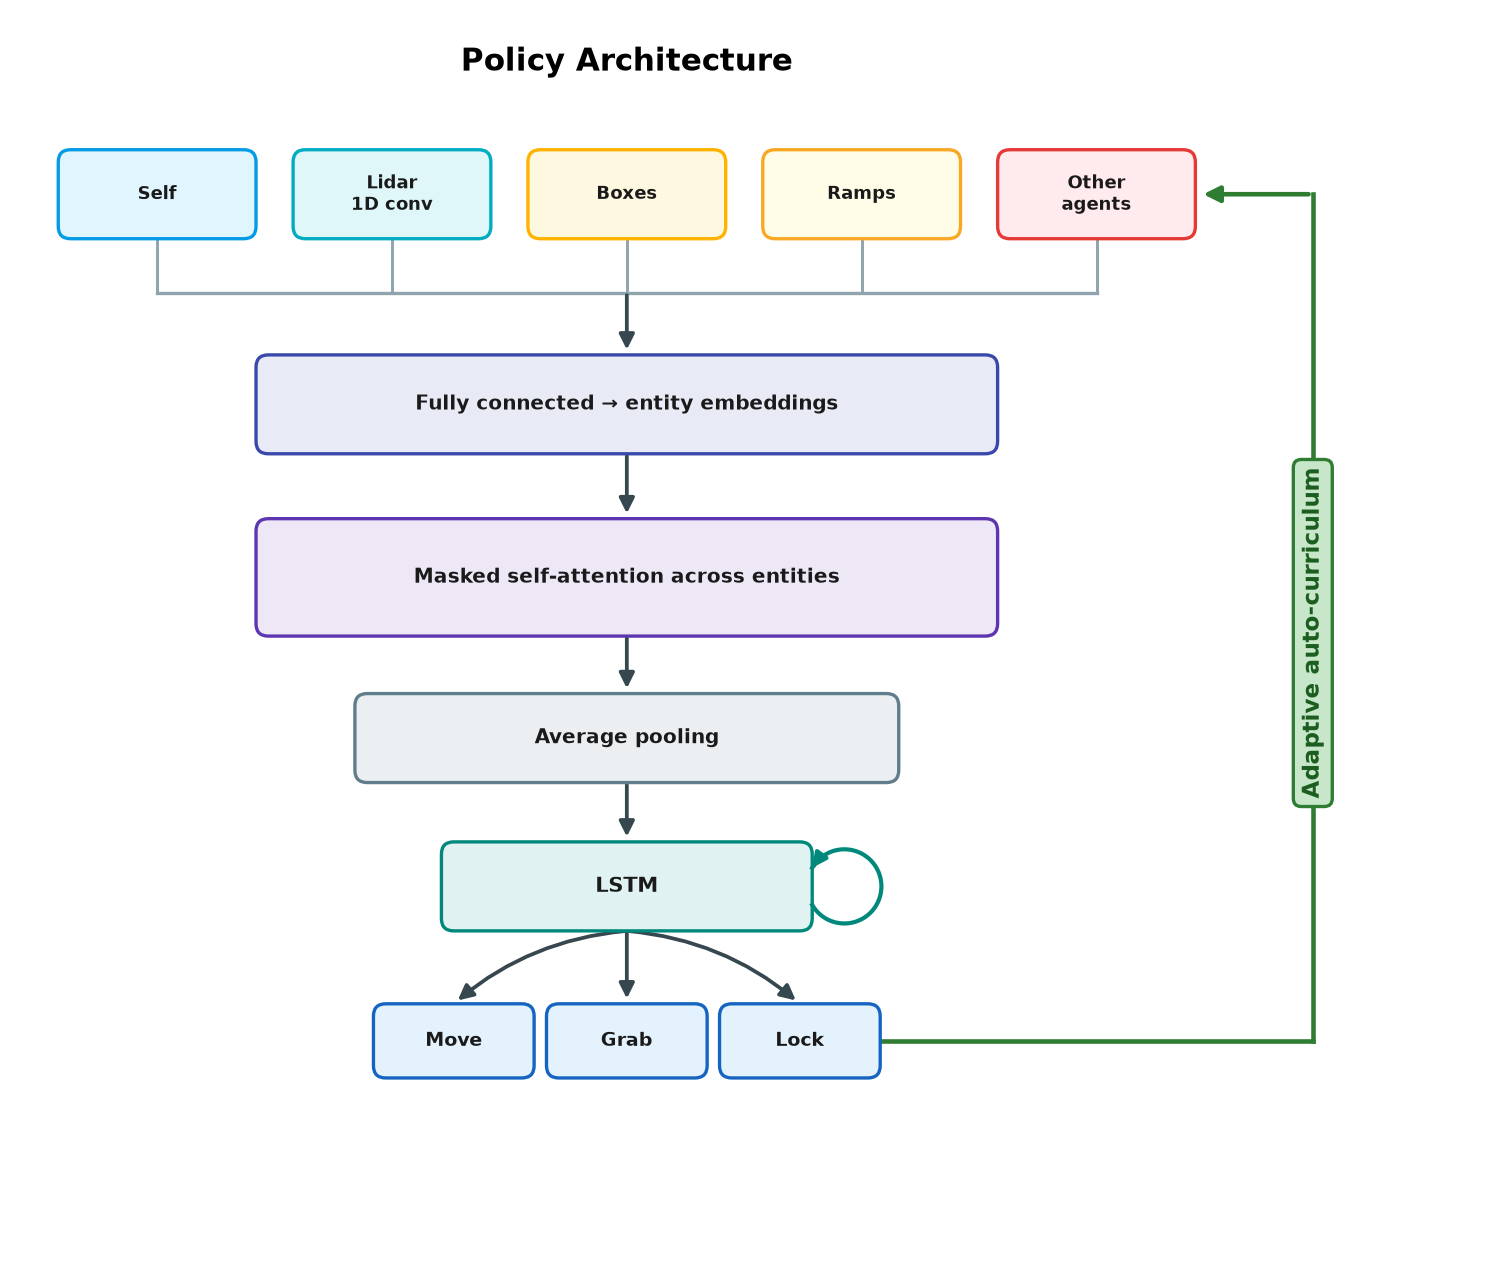
\includegraphics[width=0.75\linewidth]{images/fig_arch.png}
  \caption{Agent policy architecture. The shared
  network is trained inside an adaptive auto-curriculum, whose self-play loop
  returns the agents' own policy as their opponents.}
  \label{fig:arch}
\end{figure}

\begin{table}[H]
  \centering
  \caption{Policy architecture.}
  \label{tab:arch}
  \begin{tabular}{ll}
    \toprule
    Component & Setting \\
    \midrule
    Entity embedding dim   & 128 \\
    Self-attention         & 4 heads, 128 dim \\
    Recurrent core (LSTM)  & 256 hidden units \\
    Post-pooling dense     & 256 units \\
    Total parameters       & 1.66M \\
    \bottomrule
  \end{tabular}
\end{table}

\paragraph{Observation encoding and dimensions.}
Observations are grouped into per-entity streams, each of a fixed feature
dimension (Table~\ref{tab:obsdims}). The lidar sweep ($30$ bins) is processed by
a circular 1-D convolution ($9$ filters, kernel $3$) and flattened to $270$
features, which are concatenated with the $10$-dim self-observation to form a
$280$-dim ``main'' vector. This main vector is broadcast and concatenated onto
each entity's features before a per-stream linear embedding to $128$ dimensions,
giving encoder input widths of $290$ (agent), $292$ (box), and $289$ (ramp).

\begin{table}[H]
  \centering
  \caption{Observation streams and per-entity feature dimensions. Masked streams
  are hidden when the entity is outside the agent's line of sight.}
  \label{tab:obsdims}
  \begin{tabular}{llll}
    \toprule
    Stream & Dim (per entity) & LOS mask & Contents \\
    \midrule
    \texttt{observation\_self} & $10$        & ---               & Own pose/velocity, phase flag \\
    \texttt{agent\_qpos\_qvel} & $10$/agent  & \texttt{mask\_aa} & Other agents' pose/velocity \\
    \texttt{box\_obs}          & $12$/box    & \texttt{mask\_ab} & Box pose/velocity + lock state \\
    \texttt{ramp\_obs}         & $9$/ramp    & \texttt{mask\_ar} & Ramp pose/velocity  \\
    \texttt{lidar}             & $30\to270$  & ---               & Range sweep  \\
    \bottomrule
  \end{tabular}
\end{table}

\paragraph{How observations and dimensions affect learning.}
Two properties of this encoding are central to the emergent behaviours. First,
the line-of-sight masks (\texttt{mask\_aa/ab/ar}) remove non-visible entities
from the policy's self-attention (their attention logits are set to $-\infty$),
so the policy conditions only on what an agent can currently see---this is what
makes concealment a meaningful objective. The value network, in contrast, omits
these masks and observes all entities, yielding an asymmetric actor--critic that
stabilizes training. Second, the ramp feature dimension directly encodes the
agents' capability set: with ramp locking disabled the ramp stream has $9$
features and carries no lock state, so no policy can observe or exploit a ramp
lock. This is the single controlled change that makes ramp defense take the form
of \emph{relocation} rather than in-place locking (Section~\ref{sec:results}).

\subsection{Training: Self-Play with an Opponent Pool}
Policies are optimized with Proximal Policy Optimization (PPO)
\citep{schulman2017ppo}, maximizing the clipped surrogate objective $\mathcal{L}^{\text{CLIP}}(\theta) = \mathbb{E}_t\!\left[
    \min\!\big(\rho_t(\theta)\,\hat{A}_t,\;
    \operatorname{clip}(\rho_t(\theta),\,1-\epsilon,\,1+\epsilon)\,\hat{A}_t\big)\right],
  \rho_t(\theta)=\frac{\pi_\theta(a_t\mid o_t)}{\pi_{\theta_{\text{old}}}(a_t\mid o_t)}$, with clip range $\epsilon=0.2$, a value-function loss (coefficient $1.0$), and an
entropy bonus (coefficient $0.012$). Advantages are estimated with Generalized
Advantage Estimation (GAE) \citep{schulman2016gae}: 
$ \hat{A}_t = \sum_{l\ge 0}(\gamma\lambda)^{l}\,\delta_{t+l},
  \qquad
  \delta_t = r_t + \gamma\,V(o_{t+1})(1-d_t) - V(o_t)$, with discount $\gamma=0.998$, $\lambda=0.95$, and episode-termination flag $d_t$.
The reward is team-based and zero-sum: during the play phase hiders receive $+1$
at each step if no hider is in any seeker's line of sight and $-1$ otherwise,
and seekers receive the negation. A small penalty discourages pushing objects
out of bounds. No reward is given for any specific behaviour such as blocking a
door or using the ramp.

To stabilize self-play and mitigate strategic cycling, the opposing team is
sometimes controlled by a past snapshot, detailed below.
Table~\ref{tab:hparams} lists the training hyperparameters.

\begin{table}[H]
  \centering
  \caption{Training hyperparameters.}
  \label{tab:hparams}
  \begin{tabular}{ll}
    \toprule
    Hyperparameter & Value \\
    \midrule
    Parallel environments      & 128 \\
    Horizon (prep + play)      & 80 (32 + 48) \\
    Discount $\gamma$          & 0.998 \\
    GAE $\lambda$              & 0.95 \\
    PPO clip $\epsilon$        & 0.2 \\
    Learning rate              & $5\times10^{-4}$ (linear decay) \\
    PPO epochs                 & 4 \\
    Entropy coefficient        & 0.012 \\
    Total episodes (target)    & $43.4$M \\
    \bottomrule
  \end{tabular}
\end{table}

\paragraph{Opponent pool.}
Beginning after $10^5$ episodes, the policy is snapshotted every $10^5$ episodes
into a fixed-capacity pool holding the $N_{\text{pool}}=10$ most recent
snapshots. In each episode, with probability $p_{\text{opp}}=0.3$ the opposing
team is controlled by a snapshot drawn uniformly from the pool instead of the
current policy, otherwise both teams use the current policy. This exposes the
learner to a broader distribution of past strategies and mitigates strategic
cycling in self-play.

\subsection{Adaptive Auto-Curriculum}
Rather than hand-scheduling task difficulty, we sample the door configuration
$i\in\{0,\dots,4\}$ (each a value of $p_{\text{door}}$) with a prioritized,
replay-style curriculum inspired by Prioritized Level Replay \citep{jiang2021plr}
and the Adaptive Agent \citep{ada2023}. Each configuration keeps a learnability
score $S_i$, updated as an exponential moving average of the mean absolute GAE
advantage observed on it (a positive-value-loss / regret proxy):$ S_i \leftarrow \alpha\,S_i + (1-\alpha)\,\overline{|\hat{A}|}_i,
  \qquad \alpha = 0.9 .$
Configurations are prioritized by \emph{rank} (making the sampler
scale-invariant): if $\text{rank}(i)$ orders configurations from highest to
lowest score, the learnability distribution is
$
  P_{\text{learn}}(i) \;\propto\; \text{rank}(i)^{-1/\beta},
  \qquad \beta = 0.5 .
$
This is mixed with a staleness term favoring configurations not sampled recently
($c$ is the current episode index and $c_i$ the episode when $i$ was last
sampled), after which a floor probability $f$ is placed on the spine
configuration $i^\star$ ($p_{\text{door}}=1.0$) so that door blocking is never forgotten: 
$P(i) = (1-\rho)\,P_{\text{learn}}(i) + \rho\,\frac{c-c_i}{\sum_j(c-c_j)}$, 
where $\rho=0.3$. We then apply a small additional probability boost to the most
underrepresented phase using 
$\tilde{P}(i) = (1-f)\,P(i) + f\,\mathbf{1}[i=i^\star]$, 
where $f=0.15$.
For the first $2\times10^6$ episodes (warm-up) the sampler draws the spine
configuration with probability $0.85$ and a uniform configuration otherwise, to
bootstrap door blocking before adapting the distribution online. A newly
selected configuration is held for $20$ update batches to amortize the cost of
rebuilding the environment.

\section{Emergent behaviours}
\label{sec:results}
Training exhibits a sequence of qualitatively distinct strategies, described in
turn below. The learning curve and the behavioural figures in this section come
from a single long \emph{reference run} (our main run), which serves as an
existence proof that the full progression emerges; Appendix~\ref{app:ablation} then
shows that these dynamics are robust across seeds and causally attributable to the
adaptive curriculum. Figure~\ref{fig:curve} shows the hider win rate over
training. The curve is strongly non-monotone: it climbs to $\approx0.90$ as hiders
learn to seal the quadrant, drops sharply as seekers discover ramp use (onset
$\approx7.86$M episodes) and bottoms near $\approx0.60$ around $\approx11.29$M, and
then recovers as hiders learn to relocate and enclose the ramp, climbing back to
$\approx0.90$ by the end of training as ramp defense is mastered.
The two inflection points---the ramp-use dip and the subsequent recovery---coincide
with the phase transitions summarized in Table~\ref{tab:phases}.

\begin{figure}[H]
  \centering
  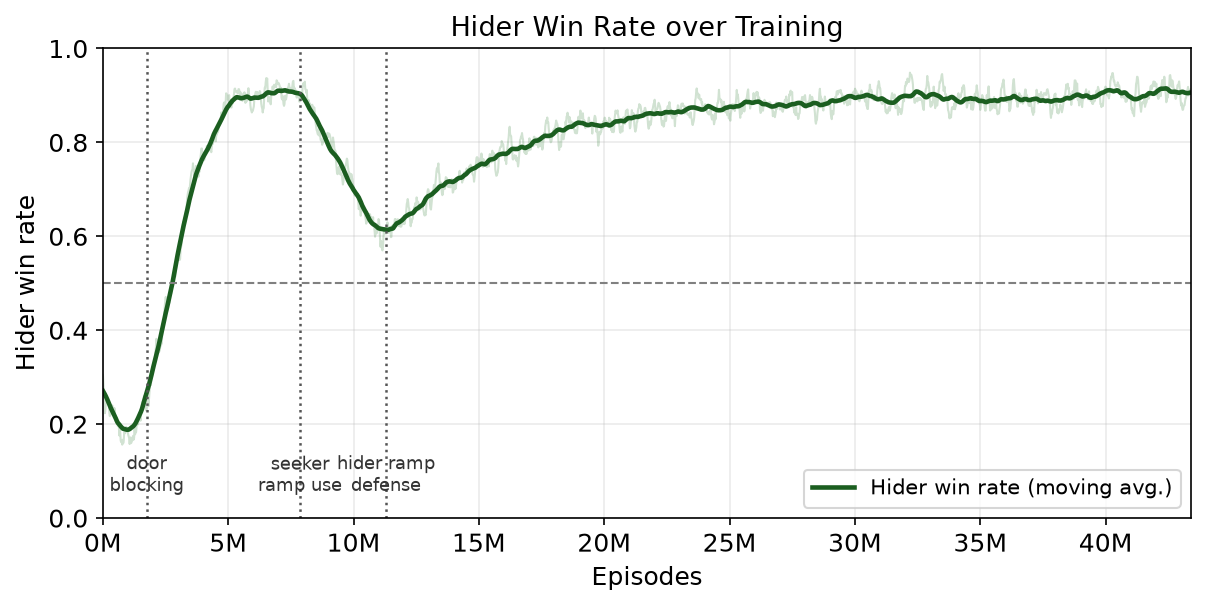
\includegraphics[width=0.78\linewidth]{images/fig_curve.png}
  \caption{Hider win rate over training. The win rate rises to
  $\approx0.90$ under door blocking, dips toward $\approx0.60$ as seekers exploit
  the ramp (onset $\approx7.86$M episodes), and then recovers, climbing back to
  $\approx0.90$ by the end of training once hider ramp defense emerges
  ($\approx11.29$M) and is consolidated.}
  \label{fig:curve}
\end{figure}

\subsection{Emergent Phases}
Training passes through four qualitatively distinct phases, described in order
below, and their approximate onsets are collected in Table~\ref{tab:phases}.

\textbf{Phase 1 --- Pursuit and evasion:}
Seekers learn to chase and hiders to flee, establishing the basic reward
gradient before any tool use appears.

\textbf{Phase 2 --- Door blocking:}
Hiders learn to move boxes into the doorway(s) during the preparation phase and
lock them, sealing the quadrant. When two doorways are open ($p_{\text{door}}<1$),
the hiders learn to block both, coordinating so that each hider seals a different
doorway rather than crowding one.

\textbf{Phase 3 --- Seeker ramp use:}
Once shelters are reliable, seekers discover (around $7.86$M episodes) that the
ramp can be moved against a wall and climbed to enter the sealed quadrant. This
corresponds to a marked drop in hider win rate, from $\approx0.90$ to
$\approx0.60$.

\textbf{Phase 4 --- Hider ramp defense:}
In response, hiders learn (from $\approx11.29$M episodes) to bring the ramp inside
the quadrant during the preparation phase and enclose it with boxes, denying
seekers the tool. The hider win rate recovers steadily and climbs back to
$\approx0.90$ by the end of training, closing the autocurriculum loop.

Every phase emerges earlier, in episode count, than the corresponding phase
reported by \citet{baker2019emergent} for the full multi-scenario environment
(door blocking $1.74$M vs.\ $\approx2.69$M, seeker ramp use $7.86$M vs.\ $8.62$M,
hider ramp defense $11.29$M vs.\ $14.5$M; Table~\ref{tab:phases}). We attribute
this acceleration to two choices: restricting training to the single quadrant
scenario, and concentrating experience on the currently-learnable door
configuration through the adaptive curriculum. The \emph{ordering} of the phases
is identical, reproducing the emergent-tool-use progression in a substantially
smaller setup.

\begin{table}[H]
  \centering
  \caption{Onset episode of each emergent phase in our quadrant reference run,
  compared with the values reported by \citet{baker2019emergent} for the full
  hide-and-seek environment.}
  \label{tab:phases}
  \begin{tabular}{lccc}
    \toprule
    Emergent phase & This work (onset) & \citet{baker2019emergent} & Improvement \\
    \midrule
    Pursuit and evasion (chasing) & $0$--$1.74$M & $0$--$2.69$M & $35.3\%$ \\
    Door blocking                 & $1.74$M      & $2.69$M      & $35.3\%$ \\
    Seeker ramp use               & $7.86$M      & $8.62$M      & $8.8\%$ \\
    Hider ramp defense            & $11.29$M     & $14.5$M      & $22.1\%$ \\
    \bottomrule
  \end{tabular}
\end{table}

\begin{figure}[H]
  \centering
  \begin{subfigure}{0.24\linewidth}
    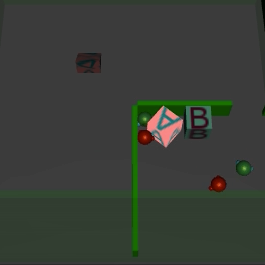
\includegraphics[width=\linewidth]{mujoco images/chasing.png}
    \caption{Chasing}
  \end{subfigure}\hfill
  \begin{subfigure}{0.24\linewidth}
    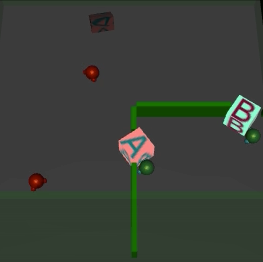
\includegraphics[width=\linewidth]{mujoco images/door blocking.png}
    \caption{Door blocking}
  \end{subfigure}\hfill
  \begin{subfigure}{0.24\linewidth}
    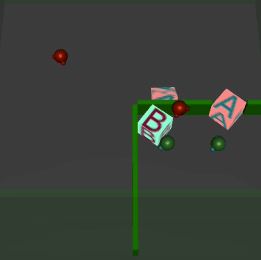
\includegraphics[width=\linewidth]{mujoco images/ramp use.png}
    \caption{Ramp use}
  \end{subfigure}\hfill
  \begin{subfigure}{0.24\linewidth}
    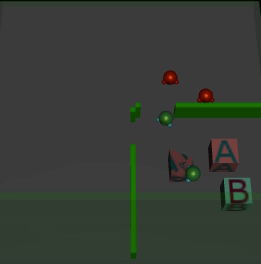
\includegraphics[width=\linewidth]{mujoco images/ramp hide.png}
    \caption{Ramp defense}
  \end{subfigure}
  \caption{Rendered snapshots of the four emergent behaviours, captured from the
  reference-run checkpoints.}
  \label{fig:snapshots}
\end{figure}

To establish that the adaptive curriculum \emph{causes} this progression rather
than merely co-occurring with it, and to characterize the coordinated object
transport and spatial strategy that implement it, we provide a controlled
curriculum ablation (Appendix~\ref{app:ablation}) together with an agent-and-box
movement analysis (Appendix~\ref{app:movement}). Further quantitative studies are
deferred to the appendix: the auto-curriculum sampling dynamics
(Appendix~\ref{app:currdyn}), a trajectory, role-assignment, and position analysis
(Appendix~\ref{app:trajectory}), and the compute-resource utilization
(Appendix~\ref{app:resources}).

\section{Sensitivity Analysis}
\label{sec:sensitivity}
To justify our two most influential design choices --- the opponent-pool size
$N_{\text{pool}}$ and the learning rate --- we sweep each in isolation (one seed
per setting) while holding all other hyperparameters fixed, and report both the
training stability and the episode at which hider ramp defense (phase~4) first
appears. Figure~\ref{fig:sens} shows the resulting learning curves and
Table~\ref{tab:sens} the phase-4 onsets.

Both sweeps single out our chosen values. With no opponent pool
($N_{\text{pool}}=0$) the hider win rate oscillates with a period of a few million
episodes as the two teams repeatedly re-exploit one another, and ramp defense does
not stabilize within budget. A pool of $5$ removes most of this oscillation but
still forgets older counter-strategies and reaches phase~4 late ($\approx18$M
episodes); $N_{\text{pool}}=10$ is the fastest and most stable ($\approx11$M),
progressing monotonically through all four phases and $N_{\text{pool}}=20$ gives
no further benefit ($\approx13$M) while doubling the snapshot memory and, through
staler opponents, slightly slowing early learning. For the learning rate,
$1\times10^{-4}$ is stable but slow (phase~4 at $\approx24$M), $3\times10^{-4}$ is
intermediate ($\approx15$M), $5\times10^{-4}$ is the fastest stable setting
($\approx11$M), and $1\times10^{-3}$ is unstable --- the policy entropy collapses,
the value loss spikes, and the win rate never settles. These sweeps identify
$N_{\text{pool}}=10$ and a learning rate of $5\times10^{-4}$ as the best-performing
configuration. These were the values we used in our main run.

\begin{figure}[H]
  \centering
  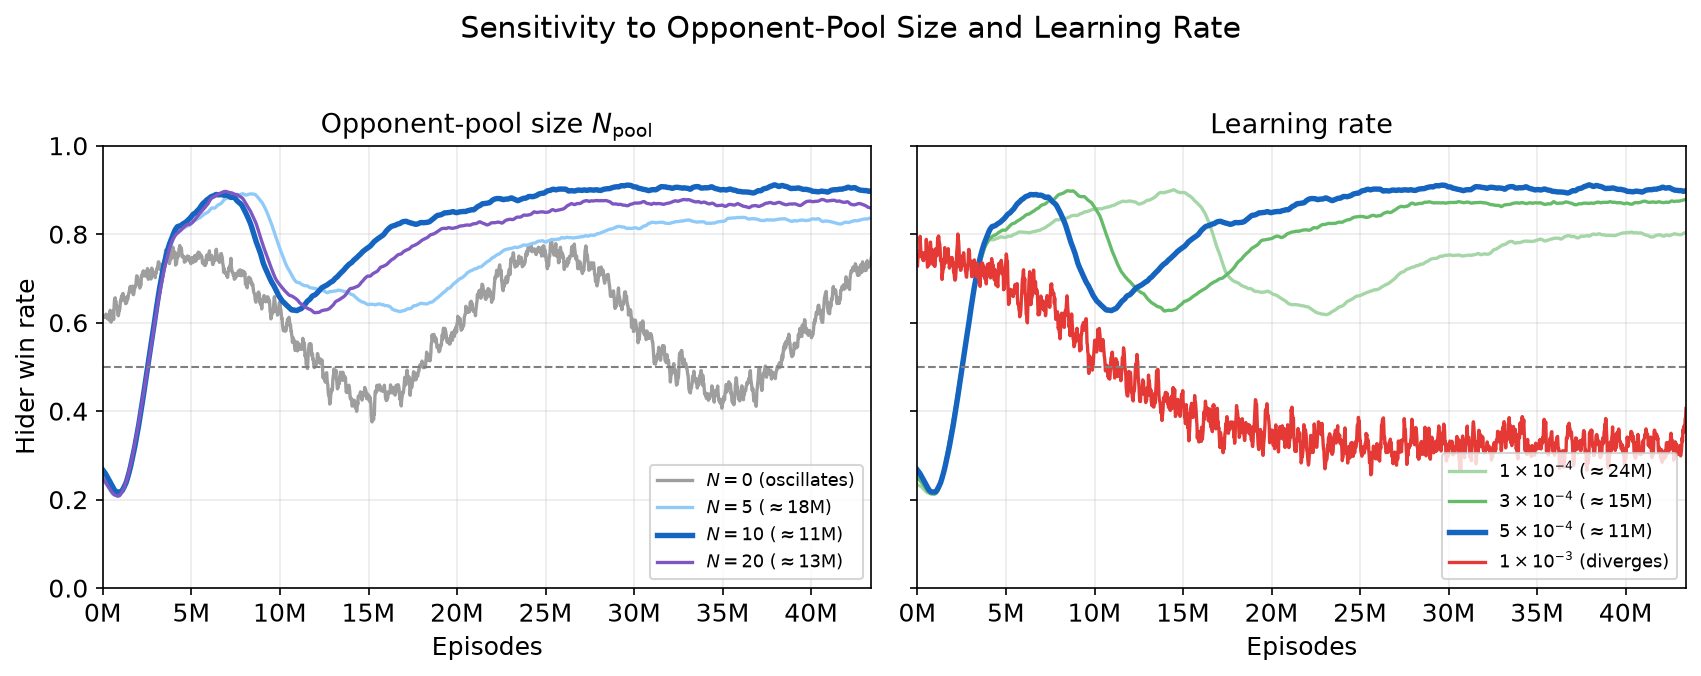
\includegraphics[width=0.98\linewidth]{images/fig_sensitivity.png}
  \caption{Sensitivity of training to opponent-pool size and learning rate.}
  \label{fig:sens}
\end{figure}

\begin{table}[H]
  \centering
  \caption{Sensitivity sweep (one seed per setting). Chosen values are
  in bold.}
  \label{tab:sens}
  \begin{tabular}{llc}
    \toprule
    Parameter & Setting & Phase-4 onset (episodes) \\
    \midrule
    Opponent pool $N_{\text{pool}}$ & $0$           & not reached \\
                                    & $5$           & $\approx18$M \\
                                    & $\mathbf{10}$ & $\mathbf{\approx11\text{M}}$ \\
                                    & $20$          & $\approx13$M \\
    \midrule
    Learning rate & $1\times10^{-4}$          & $\approx24$M \\
                  & $3\times10^{-4}$          & $\approx15$M \\
                  & $\mathbf{5\times10^{-4}}$ & $\mathbf{\approx11\text{M}}$ \\
                  & $1\times10^{-3}$          & diverges \\
    \bottomrule
  \end{tabular}
\end{table}

\section{Discussion and Limitations}
All reported behaviours emerge from a zero-sum reward with no behaviour-specific
incentives, and the only shaping is a small penalty for pushing objects out of
bounds. We emphasize that the environment and curriculum are \emph{designed} to
enable these behaviours, not to script them. The curriculum ablation of
Appendix~\ref{app:ablation} (three seeds per condition) supports a causal claim
that the adaptive curriculum accelerates and stabilizes emergence, and the
sensitivity analyses of Section~\ref{sec:sensitivity} further isolate the
opponent-pool size and the learning rate. The study is nonetheless limited to a
single scenario and a modest seed count, and further scenarios and larger seed
counts would sharpen these estimates. Finally, a promising direction for future
work is to bring recent multi-agent self-learning harnesses to bear on this
setting: in particular, the Graph-as-Policy (GaP) framework of
\citet{chen2026gap}, in which multiple agents cooperatively generate and
iteratively refine structured computation graphs, could be applied to the quadrant
scenario to compose the emergent hide-and-seek behaviours into more interpretable
and reusable policies.

\section{Conclusion}
We presented a self-contained study of emergent tool use in the quadrant
hide-and-seek scenario, driven by self-play and an adaptive auto-curriculum. The
full progression from pursuit to ramp defense emerges without behaviour-specific
rewards, with the hider ramp-defense strategy taking the form of ramp relocation.
A controlled multi-seed ablation shows that the adaptive curriculum roughly halves
the time to the final ramp-defense phase and sharply reduces its variance,
indicating that the curriculum and not just the environment, drives the reliability
of the progression.

\section*{Reproducibility Statement}
Appendix~\ref{app:software} (Table~\ref{tab:software}) lists the software
environment (language, physics engine, and key library versions) used for all
experiments. Full model and training hyperparameters are given in
Tables~\ref{tab:arch} and~\ref{tab:hparams}. All experiments use random seeds
$\{0,1,2\}$, each seeding NumPy, PyTorch, and the environment RNG. We will release
the training code, environment configuration, and per-run logs to enable full
reproduction.

\section*{Use of Large Language Models}
In this work, we used generative AI tools (large language models) to assist with implementing and debugging training and analysis code, as required for disclosure of method implementation. We did not use generative AI to generate datasets, develop the theoretical or conceptual framework, formulate or prove mathematical claims, develop hypotheses, or design the experimental methodology; these were carried out by the authors. We also used generative AI for manuscript editing, readability improvements, and drafting and polishing text. All AI-assisted code and text were reviewed, tested, and verified by the authors, who take full responsibility for the final content of this work.

\bibliographystyle{iclr2027_conference}
\bibliography{references}

\newpage
\appendix

\section*{Appendix Contents}
\vspace{0.5em}
\noindent\begin{tabular}{@{}p{2.6cm}p{8.6cm}r@{}}
\toprule
Section & Title & Page \\
\midrule
Appendix~\ref{app:ablation}    & Curriculum Ablation                      & \pageref{app:ablation}   \\[2pt]
Appendix~\ref{app:movement}    & Agent and Box Movement                   & \pageref{app:movement}   \\[2pt]
Appendix~\ref{app:software}    & Software Environment                     & \pageref{app:software}   \\[2pt]
Appendix~\ref{app:currdyn}     & Curriculum Dynamics                      & \pageref{app:currdyn}    \\[2pt]
Appendix~\ref{app:trajectory}  & Trajectory, Role-Assignment, and Position Analysis  & \pageref{app:trajectory} \\[2pt]
Appendix~\ref{app:resources}   & Computational Resource Utilization       & \pageref{app:resources}  \\
\bottomrule
\end{tabular}

\newpage

\section{Curriculum Ablation}
\label{app:ablation}
To test whether the adaptive curriculum is responsible for the emergent
progression rather than simply coinciding with it, we compare it against a
non-adaptive baseline that samples the five door configurations uniformly
(``curriculum off''), holding everything else fixed---architecture, opponent pool,
optimizer, and total budget. We train both conditions from three random seeds each
and report the mean and standard deviation. Figure~\ref{fig:ablation} shows the
hider win rate for the two conditions, and Table~\ref{tab:ablation} lists the
episode at which each emergent phase first appears.

\begin{figure}[H]
  \centering
  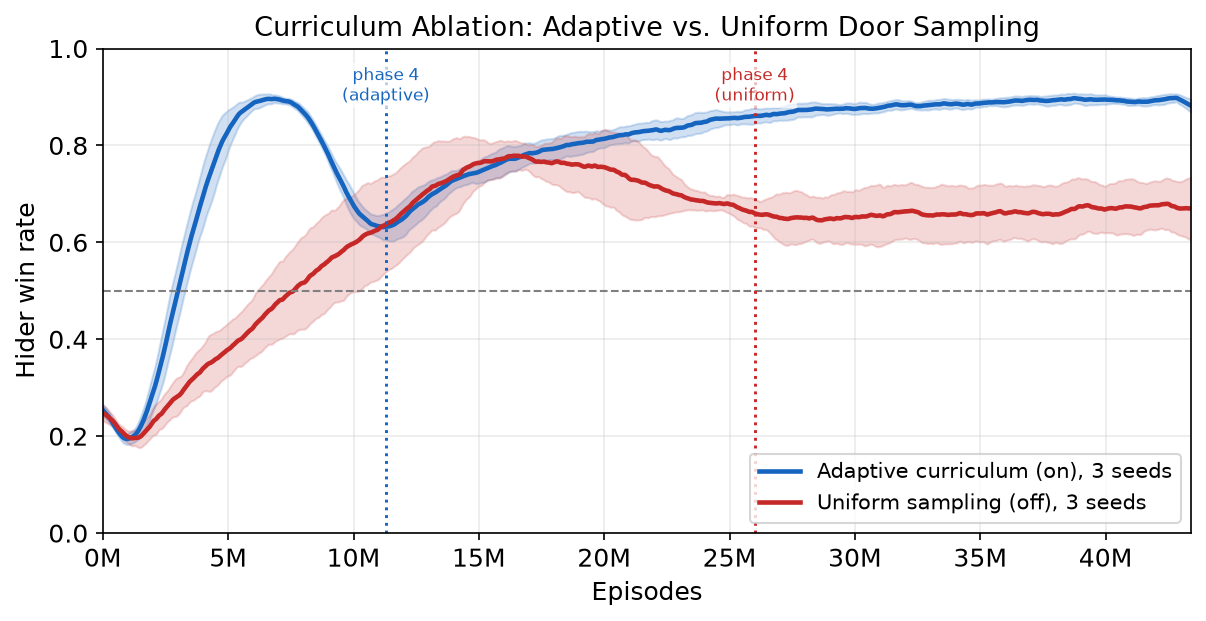
\includegraphics[width=0.8\linewidth]{images/fig_ablation.png}
  \caption{Curriculum ablation: adaptive (regret-prioritized)
  vs.\ uniform door sampling, mean $\pm$ std over three seeds.}
  \label{fig:ablation}
\end{figure}

The adaptive curriculum reaches every phase earlier and with far less variance.
Hider ramp defense (phase~4) emerges at $11.3\pm1.0$M episodes with the curriculum
but only at $26\pm6$M without it, and one of the three uniform seeds fails to
discover ramp defense within the $43.4$M-episode budget at all. Because the
adaptive curriculum surfaces the ramp-use challenge sooner, its win rate also
\emph{dips} earlier (near $8$--$11$M) than the uniform one (near $25$M), but it then
recovers faster and climbs back to $\approx0.90$ by the end of training. Within the
fixed $43.4$M-episode budget the uniform baseline reaches ramp defense too late to
fully consolidate it and plateaus lower and with a much wider band
($\approx0.67$), so the adaptive curriculum improves not only \emph{how quickly and
how reliably} the phases emerge but also the final win rate attained within budget.
The narrow $\pm1$-std band of the adaptive condition
(Figure~\ref{fig:ablation}) shows that regret-prioritized sampling also suppresses
the seed-to-seed variability that otherwise makes the timing of emergence
unpredictable.

\begin{table}[H]
  \centering
  \caption{Phase-onset episodes (mean $\pm$ std over three seeds) with and without
  the adaptive curriculum. ``(2/3 seeds)'' denotes a phase reached
  by only two of the three uniform seeds within the $43.4$M-episode budget.}
  \label{tab:ablation}
  \begin{tabular}{lcc}
    \toprule
    Emergent phase & Adaptive (on) & Uniform (off) \\
    \midrule
    Pursuit and evasion & $0.4\pm0.1$M  & $0.6\pm0.2$M \\
    Door blocking       & $1.7\pm0.3$M  & $3.4\pm0.9$M \\
    Seeker ramp use     & $7.9\pm1.0$M  & $14\pm3$M \\
    Hider ramp defense  & $11.3\pm1.0$M & $26\pm6$M~(2/3 seeds) \\
    \bottomrule
  \end{tabular}
\end{table}

\newpage
\section{Agent and Box Movement}
\label{app:movement}
Figure~\ref{fig:movement} shows agent and box displacement over a representative
episode played by a specific policy. Box motion is concentrated almost entirely in
the preparation phase: the two boxes are transported to their doorway and interior
positions within the first 32 steps.

\begin{figure}[H]
  \centering
  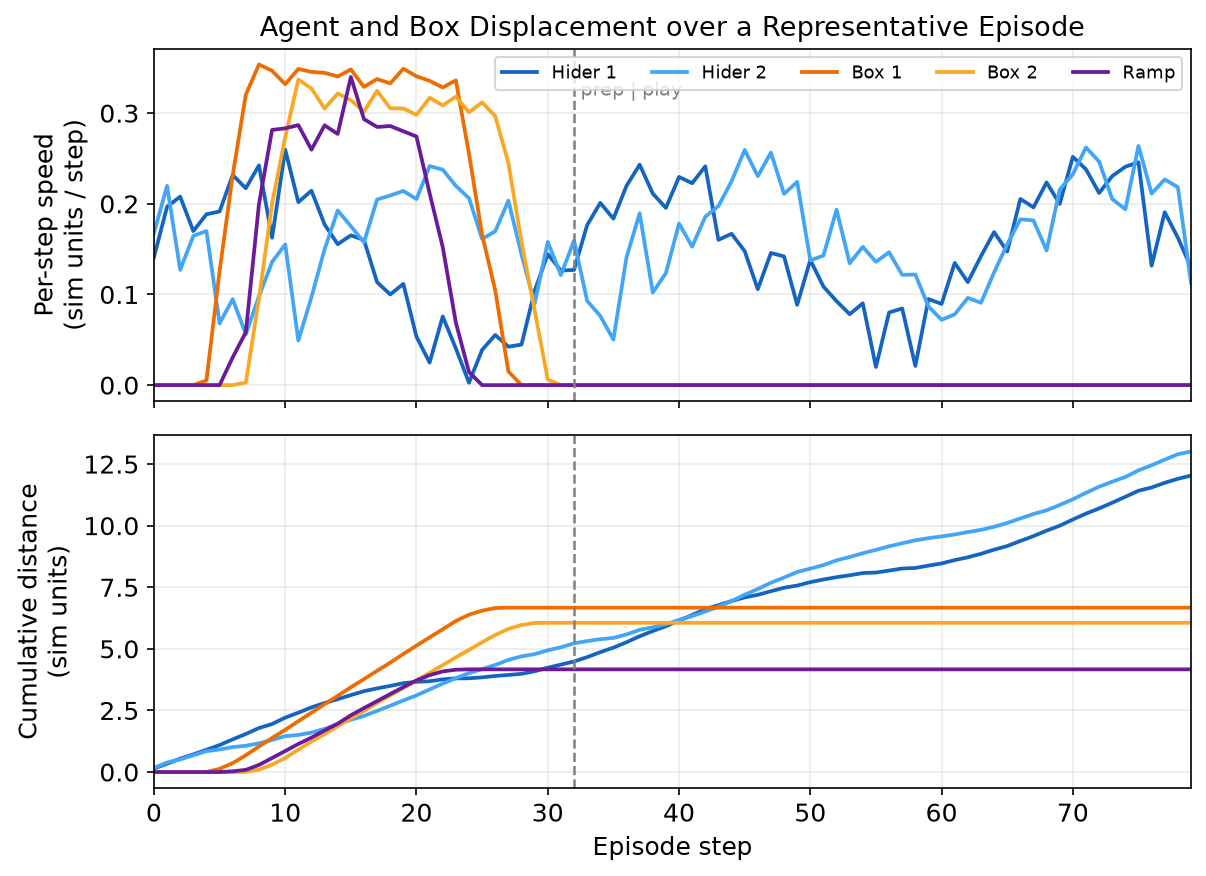
\includegraphics[width=0.75\linewidth]{images/fig_movement.png}
  \caption{Agent and box displacement over a representative
  episode.}
  \label{fig:movement}
\end{figure}

\section{Software Environment}
\label{app:software}
Table~\ref{tab:software} lists the software versions used for all experiments.

\begin{table}[H]
  \centering
  \caption{Software environment. The two environment packages
  (\texttt{mujoco-worldgen} and \texttt{mae\_envs}) are the open-source
  OpenAI repositories, installed as editable local packages.}
  \label{tab:software}
  \begin{tabular}{ll}
    \toprule
    Component & Version \\
    \midrule
    Python                     & 3.8 \\
    MuJoCo    & 1.50 (\texttt{mjpro150}) \\
    mujoco-py         & 1.50.1.68 \\
    PyTorch                    & 2.0.1 \\
    NumPy                      & 1.21.6 \\
    SciPy                      & 1.7.3 \\
    Cython                     & 0.29.36 \\
    OpenAI Gym                 & 0.15.7 \\
    \texttt{mujoco-worldgen}   & OpenAI  \\
    \texttt{mae\_envs}         & OpenAI  \\
    \bottomrule
  \end{tabular}
\end{table}

\section{Curriculum Dynamics}
\label{app:currdyn}
As a diagnostic of the curriculum itself, Figure~\ref{fig:curr} shows the
probability $\tilde{P}(i)$ with which each door configuration is sampled as a
function of the training episode. During warm-up
($<2\times10^6$ episodes) the spine configuration ($p_{\text{door}}=1.0$) dominates
at $\approx0.85$ probability, as designed. After warm-up the probability mass
shifts toward the intermediate configurations
($p_{\text{door}}\in\{0.5,0.25\}$) precisely during the ramp-use and ramp-defense
phases, because those configurations carry the highest regret while the
corresponding strategies are being acquired so the spine retains its floor
probability $f=0.15$ throughout. Late in training the distribution flattens as all
configurations approach mastery. The timing of these shifts aligns with the phase
transitions of Section~\ref{sec:results}, providing a mechanistic link between the
curriculum and the emergent behaviour.

\begin{figure}[H]
  \centering
  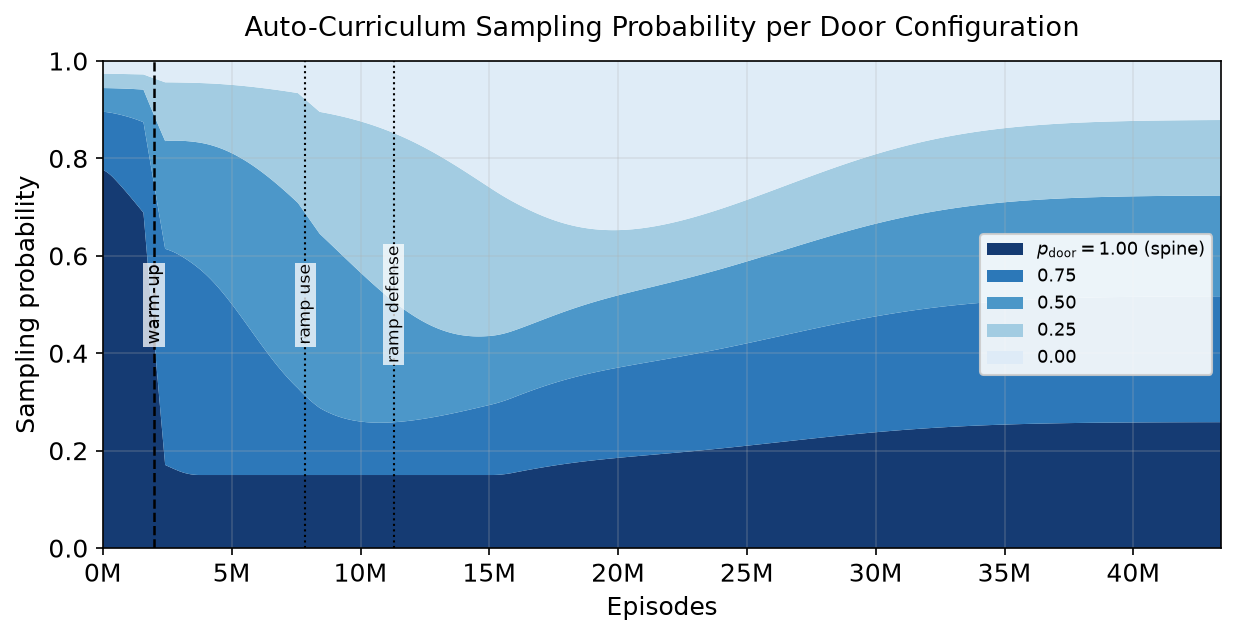
\includegraphics[width=0.70\linewidth]{images/fig_curriculum.png}
  \caption{Auto-curriculum sampling probability per door
  configuration over training.}
  \label{fig:curr}
\end{figure}

\section{Trajectory, Role-Assignment, and Position Analysis}
\label{app:trajectory}
We analyze where the two hiders go, both during the play phase---when the seal is
defended---and during the preparation phase, where the emergent strategy is
actually executed. Figure~\ref{fig:traj_ab}a tracks the two hiders' positions over a
representative winning episode: both hiders spend the play phase inside the
quadrant, with their occupancy concentrated near the sealed doorway and the
enclosed ramp rather than spread uniformly across the room, while the seekers
remain outside the quadrant for the entire play phase, consistent with a
successful seal. The corresponding preparation-phase coordination is shown in
Figure~\ref{fig:traj_ab}b: the hider that spawns closer to the ramp fetches and
relocates it into the quadrant while the other transports and locks the boxes
across the doorway. The division of labor is near-optimal and minimizes total
travel distance. When a box spawns far from the doorway, the hiders
additionally \emph{relay} it, one nudging it toward the other so that it reaches
the door in time (the ``box hand-off'' in Figure~\ref{fig:traj_ab}b).

\begin{figure}[H]
  \centering
  \begin{subfigure}{0.46\linewidth}
    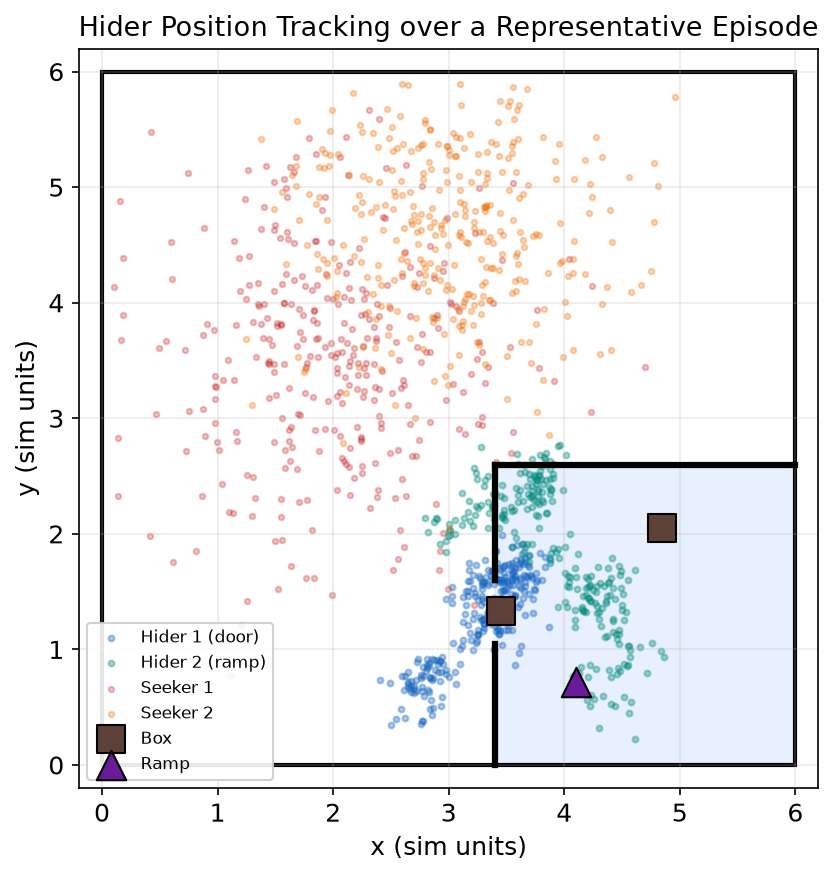
\includegraphics[width=\linewidth]{images/fig_position.png}
    \caption{Hider position tracking over a representative winning episode}
  \end{subfigure}\hfill
  \begin{subfigure}{0.46\linewidth}
    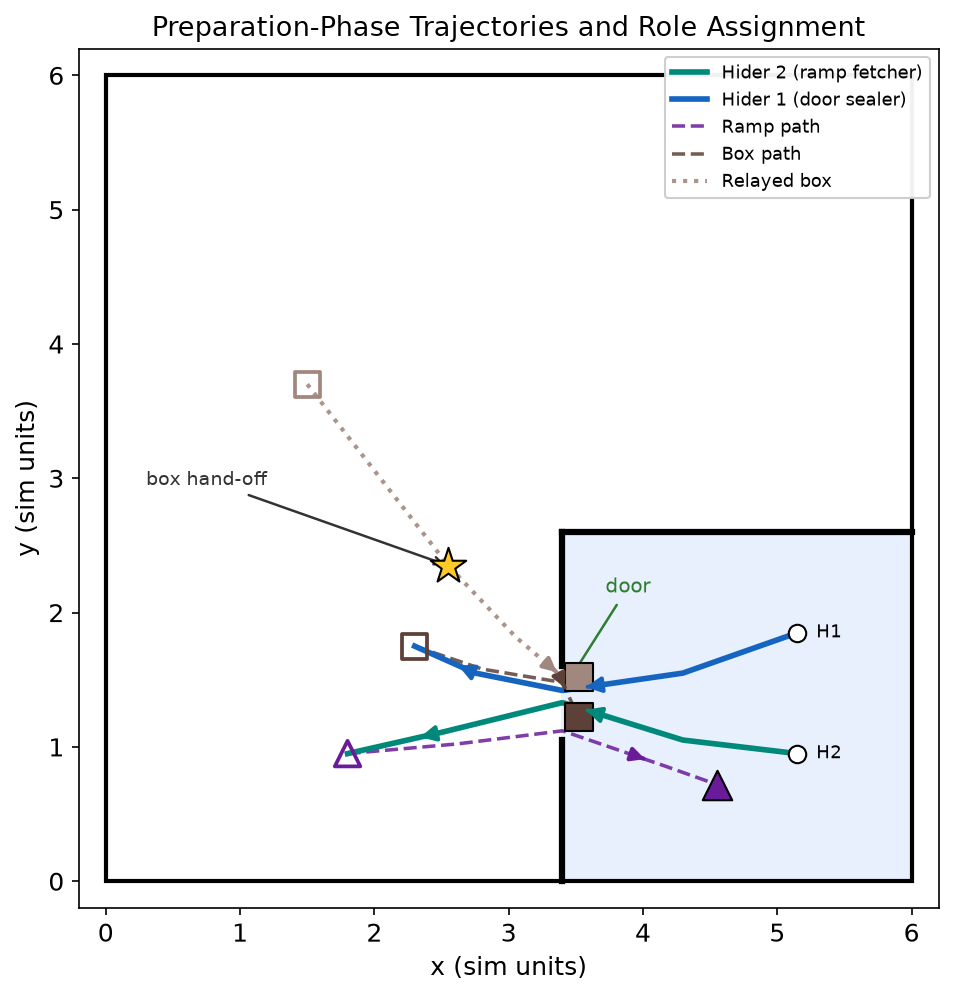
\includegraphics[width=\linewidth]{images/fig_traj_paths.png}
    \caption{Preparation-phase trajectories and role assignment}
  \end{subfigure}
  \caption{Spatial analysis of the two hiders. \textbf{(a)}~Over a representative
  winning episode the hiders' occupancy concentrates inside the quadrant, near the
  sealed doorway and the enclosed ramp, while the seekers remain outside.
  \textbf{(b)}~In the preparation phase the hider that spawns nearer the ramp
  fetches and relocates it, while its teammate seals the door.}
  \label{fig:traj_ab}
\end{figure}

Aggregated over many episodes, each hider's occupancy concentrates in a distinct
high-traffic corridor---a ``ramp corridor'' and a ``door corridor''---so the two
per-hider heatmaps are visibly different rather than interchangeable. Figure~\ref{fig:traj_heat}
shows this pattern directly: the nearer hider fetches the ramp in
$\approx88\%$ of episodes once ramp defense has stabilized, confirming that the
emergent coordination is close to distance-optimal rather than arbitrary.

\begin{figure}[H]
  \centering
  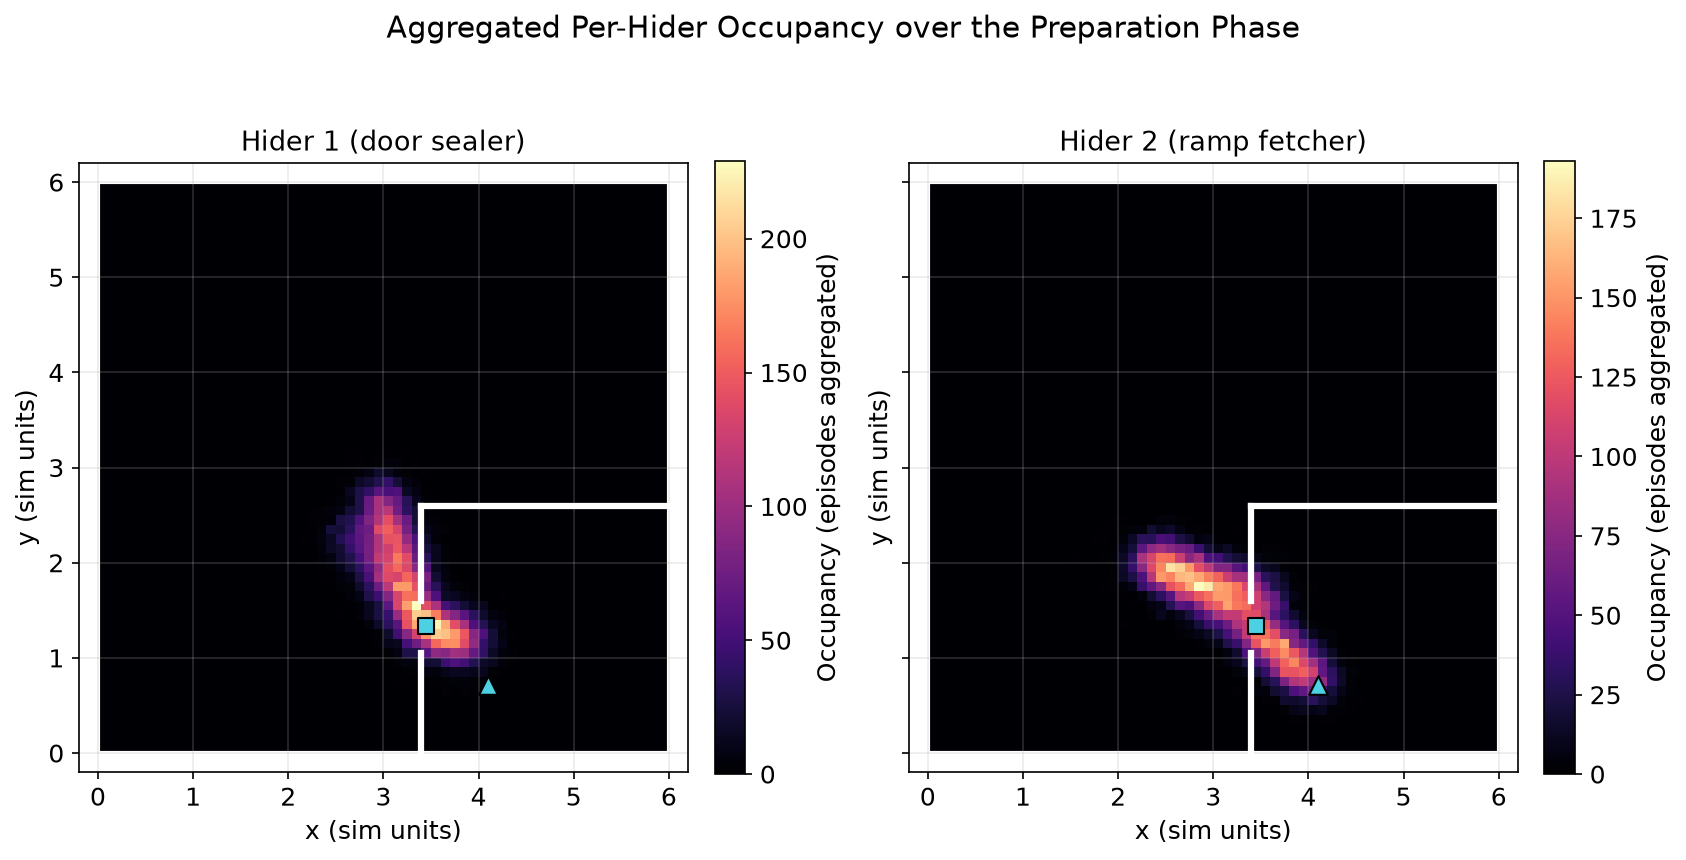
\includegraphics[width=0.8\linewidth]{images/fig_traj_heatmap.png}
  \caption{Per-hider occupancy heatmaps: door sealer vs.\ ramp fetcher.}
  \label{fig:traj_heat}
\end{figure}

\section{Computational Resource Utilization}
\label{app:resources}
We report the compute footprint of a full training run. All experiments run on a single workstation
with one NVIDIA RTX~3090 (24~GB), $32$ virtual CPU cores, and $125$~GiB of system
RAM. Table~\ref{tab:resources} summarizes utilization.

\begin{table}[H]
  \centering
  \caption{Measured resource utilization during a full training run.}
  \label{tab:resources}
  \begin{tabular}{ll}
    \toprule
    Resource & Utilization \\
    \midrule
    GPU                    & $1\times$ NVIDIA RTX~3090 (24~GB) \\
    GPU utilization        & $<10\%$ (near-idle; CPU-bound) \\
    VRAM used              & $\approx1.1$~GiB \\
    CPU                    & $32$ virtual cores \\
    Rollout workers        & $128$ ($+1$ learner process) \\
    System RAM used        & $\approx53$ / $125$~GiB \\
    Throughput             & $\approx25$ episodes/s \\
    Total episodes         & $43.4$M \\
    Total wall-clock time  & $\approx20$ days \\
    \bottomrule
  \end{tabular}
\end{table}

\end{document}
